\chapter{Introdução}
\label{cap:1intro}
\pagenumbering{arabic}

Teorias físicas permitem a realização de previsões do comportamento de um
sistema, ou seja, dada a descrição completa de um sistema físico, é possível
prever o resultado de medidas de interesse. O processo de prever o resultado é
chamado de problema direto (\textit{forward problem}). O problema de inversão
(\textit{inverse problem}) consiste em utilizar as medidas efetuadas para
inferir os valores de parâmetros que caracterizam o sistema \citep{tarantola}. O
problema direto é considerado determinístico em muitos casos. Dado o
comportamento do sistema, é possível prever o resultado da medida.
Contrariamente, o problema inverso muitas vezes não é determinístico.

Por exemplo: considere uma configuração de lâmpadas e suas potências luminosas
dentro de uma sala de aula fechada. É possível determinar a luminosidade em um
certo ponto utilizando o modelo direto, que opera sobre os parâmetros do sistema
e resulta na luminosidade em um dado ponto no espaço. O problema inverso, neste
caso, consiste em determinar a quantidade de lâmpadas e suas potências, dada a
luminosidade medida em um ou mais pontos. Claramente este problema é ambíguo,
pois existem várias configurações de lâmpadas que produzem a mesma luminosidade.
Ainda utilizando o mesmo exemplo, é possível inserir conhecimentos
\textit{a priori}, como os tipos de lâmpadas que usualmente são utilizadas em
salas de aula, para auxiliar na inversão. Num sistema real, existem ruídos que influenciam na
medida. No exemplo em questão, a sala pode sofrer entrada de luz externa e
alterar a medida num dado ponto.

\section{Problema Inverso e Incerteza}

A teoria de inversão é utilizada em diversas áreas para inferir os valores de
parâmetros relacionados com processos importantes a partir dos dados medidos,
também chamados de dados experimentais. Pode-se descrever o problema inverso
como o processo de obter informações de um sistema parametrizado, a partir de
dados observáveis, das relações teóricas dos observáveis com os parâmetros não
observáveis e do conhecimento \textit{a priori} sobre os não observáveis.

Diversas áreas precisam relacionar os parâmetros físicos caracterizando um
modelo, $m$, com medidas coletadas em um conjunto de dados, $d$. Assume-se que a
física fundamental por trás dessa relação é entendida adequadamente. Desta forma
uma função $G$ pode ser especificada para relacionar $m$ com $d$ da seguinte
forma:

\begin{equation}
\label{eq:deqgm}
d = G(m)
\end{equation}

Na prática $d$ pode ser uma função no domínio do tempo e/ou espaço, ou pode ser
uma coleção de observações discretas. Uma questão relevante é a presença de
ruído nas observações. Geralmente considera-se que os dados são observações
de um experimento perfeito $d_v$ mais uma componente de ruído $e$:
\begin{equation}
\begin{split}
d &= G(m_v) + e \\
&= d_v + e
\end{split}
\end{equation}
onde $d_v$ satisfaz  \ref{eq:deqgm} para o modelo considerado verdade $m_v$, 
$d_v = G(m_v)$, assumindo o operador $G$ como exato. Em muitos casos é possível
ajustar matematicamente todas as partes do ruído $e$ utilizado a equação \ref{eq:deqgm},
deixando o ruído aparecer no modelo encontrado. Situação que na prática é
indesejável, pois em muitos casos uma solução de $m$ que é influenciada por até
mesmo um pequeno ruído $e$ pode ter pouca similaridade com o modelo verdadeiro
$m_v$ \citep[p. 19]{aster2013parameter}.

Dada a natureza dos problemas de inversão mais complexos, encontrar
matematicamente modelos que expliquem os dados não é suficiente para
caracterizar qual solução foi obtida e o quão próxima ela está do modelo
verdadeiro $m_v$, o quão boa é em termos de plausibilidade física e se é
consistente com outras restrições do problema. Os principais desafios
encontrados em problemas de inversão que precisam ser considerados e também
levam à incerteza no resultado são:

\begin{itemize}
  \item Existência. Pode não existir um modelo que ajuste exatamente aos dados,
  devido à aproximações feitas no modelo físico ou porque os dados contém ruído.
  \item Unicidade. No caso de existir solução exata, ela pode não ser única,
  mesmo para um número infinito de observações. Ou seja, podem existir outros
  $m$ além $m_v$ que satisfazem $G(m)=d_v$. Esta questão gera a estimativa de
  modelos suavizados em relação à realidade, o que é estudado pelo tópico de
  análise de resolução.
  \item Instabilidade. O processo de computar uma solução inversa geralmente é
  instável pois pequenas mudanças nos dados $d$ podem gerar grandes mudanças no
  modelo estimado. Problemas em que esta situação ocorre são ditos mal postos ou
  mal condicionados. Para contornar esta questão, restrições adicionais devem
  ser impostas, as quais adicionam viés à solução para incorporar os
  conhecimentos \textit{a priori}, procedimento chamado de regularização.
  \item Regularização: Informações adicionadas para restringir o resultado de
  moto a integrar o conhecimento \textit{a priori} são incertas, pois são
  baseadas no conhecimento e experiência do especialista.
\end{itemize}



\section{Inversão Sísmica}

No contexto da indústria de óleo e gás, o problema de inversão sísmica é
importante para o processo de caracterização de reservatórios de
hidrocarbonetos, que consiste na determinação tridimensional e quantitativa da
estrutura e das propriedades petrofísicas (porosidade, densidade, etc) das
rochas da subsuperfície. O método de aquisição sísmica de reflexão utiliza
pulsos sísmicos de uma fonte artificial controlada e monitora a resposta em
função do tempo. Neste sistema, cada interface entre dois tipos de rochas
diferentes gera reflexão e refração do pulso sísmico, como demonstrado na Figura
\ref{fig:1sismica}.

\begin{figure}[ht!]
\begin{center}
  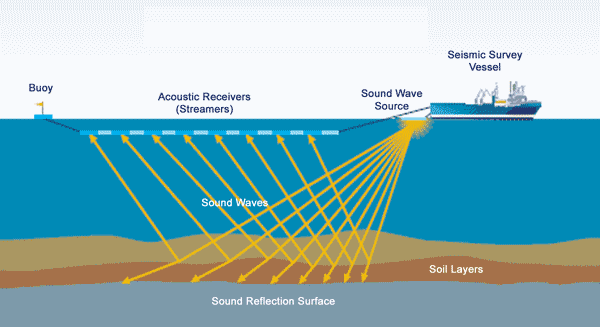
\includegraphics[width=0.8\textwidth]{fig/seismic_survey}
  \caption{Método de sísmica de reflexão \citep{figsismica}}
  \label{fig:1sismica}
\end{center}
\end{figure}


Para inversão acústica, o modelo mais utilizado para representar a resposta do
pulso sísmico atravessando as interfaces entre rochas é o convolucional. Nele é
assumido um modelo em camadas para a subsuperfície e ângulo de incidência e
reflexão de $90^\circ$. A medida efetuada é representada pelo resultado da
convolução do pulso sísmico, também chamado de \textit{wavelet}, com as
refletividades das interfaces. Os coeficientes de reflexão com ângulo de
reflexão normal são modelados por \citep[p. 69]{sen_livro}:

\begin{equation}
r(t) = \frac{z(t+\delta t)-z(t)}{z(t+\delta t)+z(t)}
\end{equation}
onde $z(t)$ é a impedância acústica no tempo $t$ definida por
$z(t)=\rho(t)v(t)$, onde $\rho(t)$ é a densidade da rocha e $v(t)$ a
velocidade de propagação da onda acústica. Utilizando os coeficientes de
reflexão, modela-se a resposta do sistema $d(t)$ aplicando a convolução
da \textit{wavelet} $s$ com os coeficientes de refletividade:

\begin{equation}
d(t) = \int_{-\infty}^{\infty} s(\tau)r(t-\tau)d\tau + e_d(t)
\end{equation}
onde é assumida a presença de um ruído aleatório $e_d(t)$ e $d$ é o chamado dado
sísmico. Cada sequência de dados $d$ representa um ponto no plano $xy$ e suas
posições $(t)$ são coordenadas em tempo que se relacionam com a profundidade.
Cada $d_{xy}$ é muitas vezes chamado de traço sísmico, o que no caso discreto
pode ser uma coluna de uma matriz 2D, por exemplo. Um conjunto de traços
sísmicos também é chamado de uma imagem, seção ou cubo, no caso de um
levantamento 3D. A \textit{wavelet} ideal seria um pulso tipo delta contendo
todas as frequências, mas gerar tal pulso não é viável. Na prática as
\textit{wavelets} são pulsos de banda limitada entre $6Hz$ e $65Hz$, o que
limita a frequência da sísmica e sua resolução \citep[p. 11]{sen_livro}.
A Figura \ref{fig:wavelet} ilustra uma \textit{wavelet} típica extraída de dados
reais.

\begin{figure}[htp]
\begin{center}
  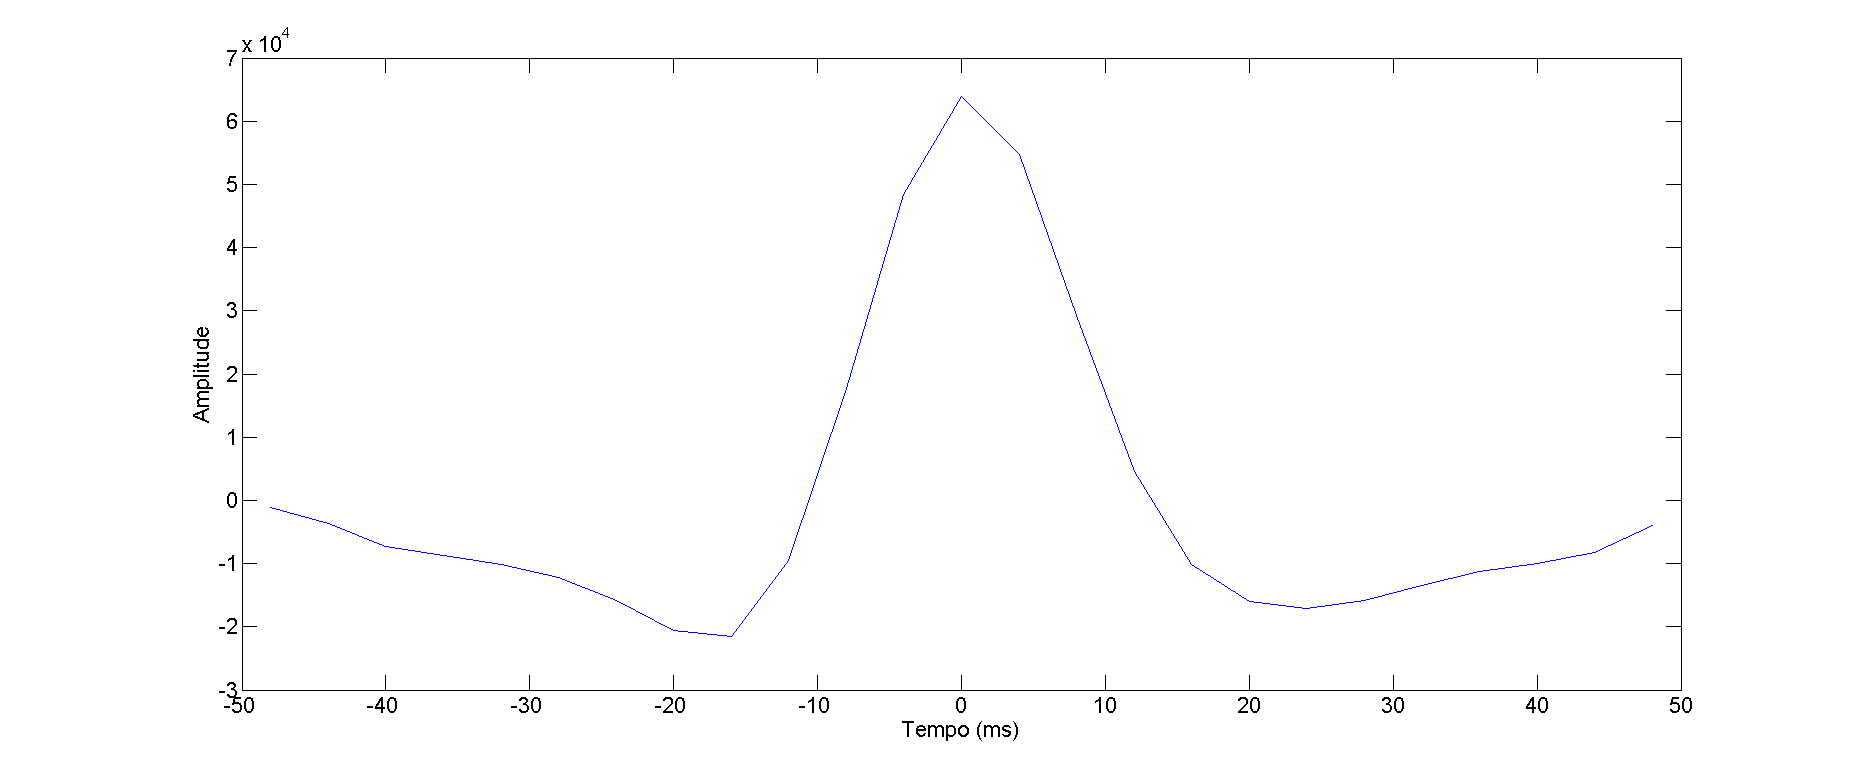
\includegraphics[width=0.8\textwidth]{fig/wavelet}
  \caption{\textit{Wavelet} extraída de dados reais}
  \label{fig:wavelet}
\end{center}
\end{figure}

O objetivo da inversão sísmica acústica é determinar os valores de impedância
acústica das camadas de rocha. Esse é um problema não linear, pois as equações
que determinam o modelo direto são não lineares. Também é considerado mal posto,
pois é ambíguo, ou seja, várias combinações de camadas e suas impedâncias podem
gerar o mesmo resultado no dado sísmico. Essas características geram a
necessidade de alta intervenção de especialistas para restringir o resultado
(regularização). Quando poços são perfurados, são utilizadas outras ferramentas
para observar dados mais próximos aos reais. Os principais métodos de inversão
utilizam os dados de poços para regularização e geração de estatísticas.

No processo de inversão é importante a modelagem da incerteza dos resultados
obtidos, ou seja, obter soluções equivalentes respeitando os dados medidos e as
informações \textit{a priori}. Essas soluções devem representar bem a região
onde o erro é menor que a tolerância desejada, chamada de região de equivalência
\citep{tompkins_comparisonBayes}. Existem várias razões para essa região de
equivalência existir, incluindo erros nas medidas, cobertura dos dados sobre a
as localizações desejadas, limitação de banda do pulso sísmico, suposições sobre
o modelo físico (e.g. isotropia, modelo de camadas, homogeneidade, etc.) e
aproximações matemáticas do modelo direto. A modelagem de incerteza ajuda na
avaliação dos riscos envolvidos nos processos de perfuração, exploração e
produção de óleo e gás.

As médias e variâncias locais das soluções não são suficientes para caracterizar
a incerteza na inversão, pois os modelos de impedância geralmente são utilizados
como entrada de processos como a simulação de fluxo. Esse tipo de simulação é
essencialmente uma função não linear, ou seja, a média das simulações de fluxo
não é necessariamente igual a simulação da média das impedâncias:
$F(\overline{\mathbf{m}})\neq \overline{F(\mathbf{m})}$, onde ${\mathbf{m}}$
representa as soluções aceitáveis, $F(\cdot)$ a função não linear da
simulação de fluxo e $ \overline{(\cdot)}$ a operação de média. Amostragem, de
uma forma geral, possibilita análises mais sofisticadas da distribuição
posterior \citep{hansenGibbsPrior}.

%TODO importancia das realizações na modelagem, ainda falta citação da
% simulacao de fluxo (funcao nao linear)

 Na literatura recente, diversos métodos foram propostos para tentar solucionar
 o problema da inversão sísmica com modelagem de incerteza.
Modelos envolvendo técnicas de inteligência computacional foram propostos para
tentar resolver o problema
\citep{senSimulatedAnnealin,MallickGeneticInve,max_inv_simulated,Artun2011143,MartinezPSO,Sambridge22102013}.
Apesar de terem oferecido bons resultados, esses modelos baseados em otimização
não capturam de forma ideal o conhecimento do especialista. A incerteza
resultante desses métodos é relacionada com o nível em que foi explorada a
superfície de erro, ao invés da incerteza relacionada aos dados e conhecimentos
\textit{a priori} inseridos.

O uso de ferramental probabilístico baseado no teorema de Bayes pode ser
aplicado, em conjunto com o amostrador de Gibbs, para gerar realizações
estocásticas da distribuição \textit{a posteriori} \citep{leandro_SEG}. Assim,
pode-se computar estatísticas do conjunto de soluções, obtido à alto custo
computacional. Para atacar a maldição da dimensionalidade e diminuir o custo da
amostragem de soluções, foram propostos métodos que utilizam redução dimensional
\citep{TompkinsScalabUnce2011}. Neste caso, aplicando análise de componentes
principais (PCA) é possível reduzir a dimensão do problema e utilizar um esquema
de amostragem determinística, ao custo de perda na resolução espacial das
amostras.


% amilcar aqui
A área de Geoestatística teve início a partir do uso de ferramentas estatísticas
para tratar dados espaciais, modelar suas continuidades e lidar com incertezas
presentes nos problemas da Geologia \citep[p. 3]{isaaks1989geostats}. Antes de
sua criação, um atributo de rocha, por exemplo, era tratado como se fosse uma só
variável aleatória. Ou seja, os valores desse atributo nos pontos espaciais de
uma área eram tratados como amostras de uma mesma distribuição de probabilidade.
A Geoestatística passou a assumir a característica espacial dos dados, onde cada
posição da área é tratada como uma variável aleatória possuindo correlações com
suas vizinhas.

\cite{amilcarInversao} propõem um método de inversão, chamado \textit{Global
Stochastic Inversion (GSI)}, baseado em \textit{Direct Sequential Simulation}
(DSS), uma importante ferramenta da Geoestatística. Na DSS são utilizados
modelos de continuidade direcional dos dados (variogramas direcionais, ou
funções de correlação) para simular pontos não observados da área, respeitando
assim a continuidade espacial, a variabilidade e o histograma observados nos
dados de poços. O processo de inversão faz uso de DSS  para encontrar um
conjunto de soluções que tenha alta correlação com o dado sísmico. Apesar da
vantagem de se modelar a continuidade espacial em quaisquer direções desejadas,
o método foi concebido para trabalhar em áreas pequenas, pois assume a estacionariedade
das médias. Além disso, não converge em problemas mais avançados como a inversão
para dados de porosidade \citep{amilcarInversao}.

\section{Objetivo}

O objetivo do presente trabalho consiste em propor um modelo capaz de integrar a
atualização Bayesiana no processo de inversão GSI. Resultados prévios indicam
que utilizar o método determinístico de inversão Bayesiana
\citep{Buland01012003}, como base para iniciar a DSS, obtém maior correlação com
a sísmica na primeira iteração da GSI. Com o novo modelo espera-se aumentar a
eficiência da amostragem comparada à Bayesiana e aplicar o método em inversão
para outras propriedades de rocha além de impedância acústica. A modelagem da
continuidade espacial é outra vantagem que se espera obter ao se integrar as
propostas. No modelo de amostragem Bayesiana atual é inviável computacionalmente
modelar a continuidade em direções que não sejam a vertical, pois para tanto é
necessário inserir as covariâncias entre todos os pontos a serem invertidos.

Outro objetivo é integrar ao modelo, durante o processo de inversão, a
metodologia descrita em \cite{caers_distance_kernels_MDS}, na qual as incertezas
relativas aos dados de entrada considerados como certos podem ser analisadas,
afim de verificar a sua influência na modelagem de incerteza do resultado da
inversão.


\section{Organização do Texto}

Este documento está organizado da seguinte forma. Após esta breve introdução, o
Capítulo \ref{cap:2modelosInversao} apresenta o estado da arte em modelos de
inversão sísmica com modelagem de incerteza. O Capítulo \ref{cap:3modeloHibrido}
trata da proposta do projeto e resultados preliminares da integração de
atualização Bayesiana em inversão Geoestatística, a ser desenvolvido em parceria
com o CERENA - Centro de Recursos Naturais e Ambiente do Instituto Técnico da
Universidade de Lisboa, sob orientação do professor Dr. Amilcar Soares,
especialista em Geoestatística e inversão sísmica. O estágio será iniciado em
julho de 2015 e terá 12 meses de duração. Após o retorno ao Brasil, estão
planejados mais 8 meses de trabalho para finalizar a escrita da tese e defesa.

